\begin{frame}[fragile]{PresustentacionesAWPS: un servicio, dos contratos}
\begin{columns}[T]
\begin{column}{0.4\textwidth}
\small
\begin{itemize}
\item Ya tenía REST: 20 controladores, JWT y Swagger.
\item Nuevo: SOAP con Spring Web Services y WSDL en \texttt{/ws/estado.wsdl}.
\item Reutiliza \texttt{EstadoConsultaService}: la lógica no se repite.
\item 119 pruebas pasan; 2 son del SOAP.
\end{itemize}
\end{column}
\begin{column}{0.56\textwidth}
\begin{lstlisting}
@PayloadRoot(namespace = NAMESPACE,
    localPart = "ConsultarEstadoSolicitudRequest")
@ResponsePayload
public ConsultarEstadoSolicitudResponse consultarEstado(
        @RequestPayload ConsultarEstadoSolicitudRequest peticion) {
    Map<String, Object> estado = estadoConsultaService
        .obtenerEstadoSolicitud(peticion.getSolicitudId());
    if (!estado.containsKey("solicitudId")) {
        throw new SolicitudNoEncontradaException(
            peticion.getSolicitudId());
    }
    ...
}
\end{lstlisting}
\end{column}
\end{columns}
\end{frame}

\begin{frame}{La misma consulta por REST y por SOAP}
\centering
\IfFileExists{../figuras/benites-peticiones.png}{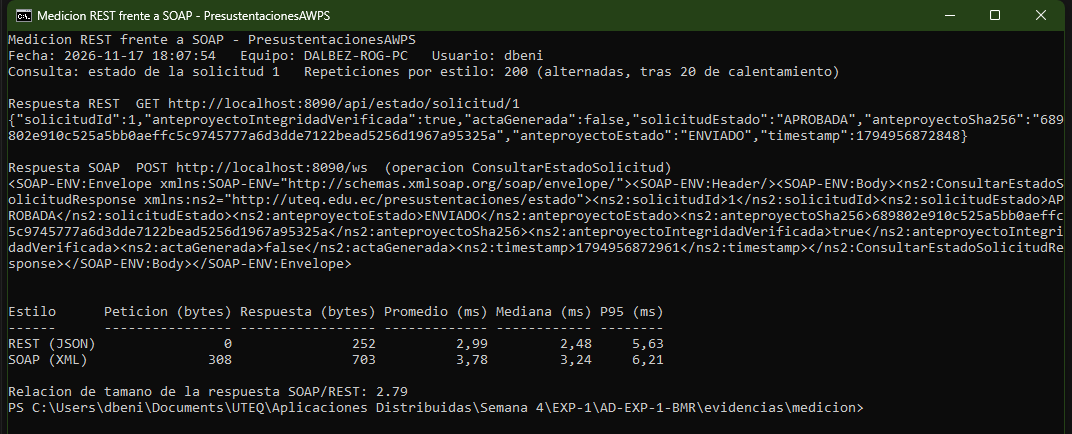
\includegraphics[width=0.95\linewidth,height=0.74\textheight,keepaspectratio]{../figuras/benites-peticiones.png}}{\fbox{\parbox[c][4.5cm][c]{0.85\linewidth}{\centering\color{gris}Falta \texttt{figuras/benites-peticiones.png}: captura de la terminal con la medición}}}
\end{frame}

\begin{frame}{Medición propia: REST frente a SOAP}
\begin{columns}[c]
\begin{column}{0.56\textwidth}
\footnotesize
\begin{tabular}{@{}lrr@{}}
\toprule
 & REST & SOAP \\
\midrule
Petición, cuerpo (bytes) & 0 & 308 \\
Respuesta (bytes) & 252 & 703 \\
Promedio (ms) & 2,99 & 3,78 \\
Mediana (ms) & 2,48 & 3,24 \\
Percentil 95 (ms) & 5,63 & 6,21 \\
\bottomrule
\end{tabular}
\par\vspace{6pt}
{\scriptsize 200 consultas por estilo, alternadas, en la misma PC y sin red (17/11/2026). Script y resultado en \texttt{evidencias/medicion}.\par}
\end{column}
\begin{column}{0.4\textwidth}
\cifra{2,8 veces}{más bytes en la respuesta SOAP}
\vspace{10pt}
\cifra{+0,79 ms}{por consulta con SOAP, en promedio (26\,\% más)}
\end{column}
\end{columns}
\vspace{10pt}
\begin{block}{Qué nos dice}
Para el \emph{polling} de Angular cada 15 segundos conviene REST: menos bytes y menos tiempo. SOAP vale la pena cuando otro sistema necesita un contrato WSDL formal.
\end{block}
\end{frame}
